\chapter{Concept and Design}
\label{cha:conceptanddesign}

\section{General}

\section{Requirements and Challenges}

\subsection{Requirements}

\subsubsection{GDPR compliance}
The General Data Protection Regulation (GDPR) is a regulation by the European Parliament, Council of the European Union and the European Commission focussed on strengthening EU citizens digital privacy.  Its main focus is on giving citizens control over their digital personal information and simplyfying the regulatory environment for multinational corporations. However it also adds a strict data compliance regime, by penalizing transgressions with up to 4\% worldwide turnover. Furthermore this regulation does not have to be verified by each EU's regulatory body, since it is a EU regulation, compared to an EU directive which has to be ratified by each EU signatory state.

\section{Processes}

\subsection{Registration}
In order to be part of our distributed digital identity system that we envisioned, it is necessary to register with it first. The registration process consists of the following steps (See Figure \ref{fig:registration_concept}):

\begin{enumerate}
\item \label{registrar_item_one}
The user creates an ethereum address and a private public key pair, the combination of these two are now used as the users digital identity. Jointly they can be used as a digital identity card. They are safely and securely stored in the users own database.
\item \label{registrar_item_two}
For verification and auditing purposes these have to be verified by a trusted party, so that third parties can be sure of the identity of the individuals. We are using a specially designed smart contract, where the user inputs his ethereum address and his public key. Once filled, he writes it to the blockchain and waits for the trusted party, in our case a governmental agency, to check the contents, fulfill and sign the contract.
\item \label{registrar_item_three}
The user now verifies himself using the eID online verification system. After successfully verifiying he sends the governmental agency, entrusted with handling digital identity services, his ethereum address and public key. These are used for the upcoming smart contract verification.
\begin{comment}
DONT NEED: The user can now have his ethereum address and private public key pair verified by a governmental agency.
\end{comment}
\item \label{registrar_item_four}
The aforementioned governmental agency can now check the blockchain for the requesting users registrar contract, verify its content against already received (See \ref{registrar_item_three}) or saved information and then link the existing user to the ethereum address and public key. After extending the database entry the agency now collects all existing claims for that individual, packages them into a single claims object and sends it to the user for his record keeping and claim query construction.  
\item \label{registrar_item_five}
Lastly the agency signs and approves this registrar contract. By adding its signature the user is now a fully registered member within our community. Henceforth he can use this identity to request services and offer claims to and from other registered parties. 
\end{enumerate}

\begin{figure}[ht]
\centering
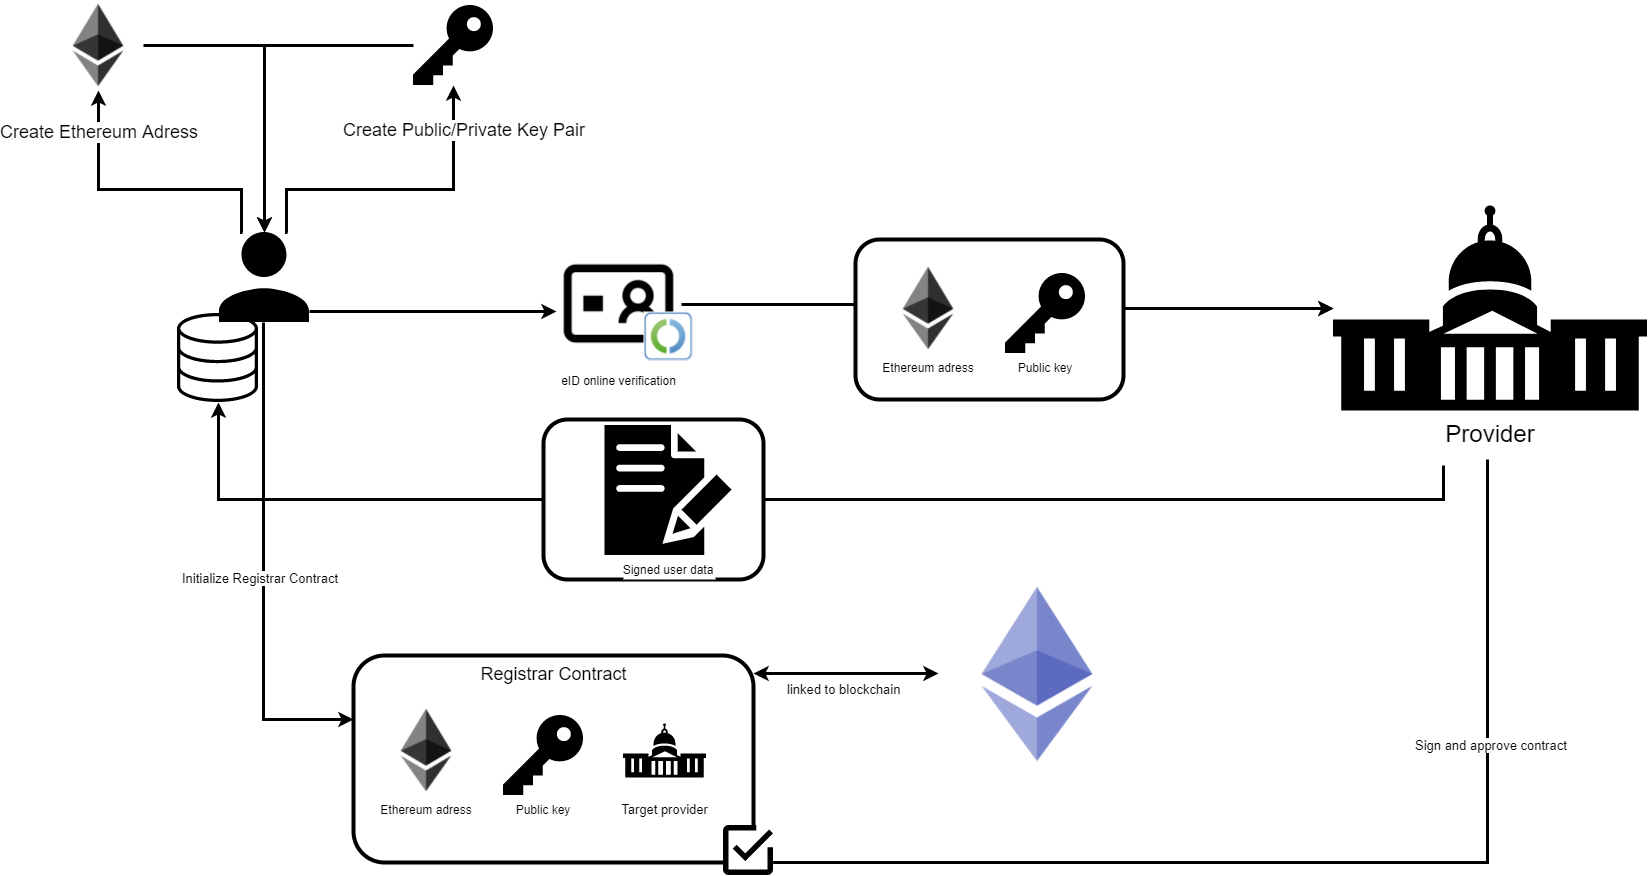
\includegraphics[width=\textwidth]{concept/registration.png}
\caption{Registration}
\label{fig:registration_concept}
\end{figure}

\subsection{Permission Request}
After registration the user is now able to use \projectName{} for identification and verification purposes. Lets consider opening a new bank account using \projectName() for verification.



\begin{enumerate}
\item \label{permission_request_item_one}
We have a user called Tom who has just recently moved and is interested in opening a new bank account for his local dealings. He therefore visits a local branch of Bank X and requests a new bank account. He now hands his ethereum address, public key, Name, Address etc. to the bank teller.
\item \label{permission_request_item_two}
The bank teller now enters that information into a \textbf{Request Permission} form and sends it to the government for verification purposes.
\item \label{permission_request_item_three}
The government now writes a new permission request contract into the ethereum blockchain. This contract contains the following information:
\begin{itemize}
\item @EthereumAddress; This is Toms Address, as his information is requested
\item ThirdPartyName; This is the requesting Party's Name Bank 
\item AttributesRequested[GivenName, FamilyName, StreetName, StreetNumber, PostalCode, DateOfBirth, ...]; This is an Array containing all Variables requested by the Third Party
\end{itemize}
\item \label{permission_request_item_four}
The user now polls the blockchain for new messages and finds this permission request by the third party.
\item \label{permission_request_item_five}
Tom now checks each requested attribute and selects the attributes he wants to share with the third party. After his selection a specific query is created imitating his choices.
\end{enumerate}

\begin{figure}[ht]
\centering
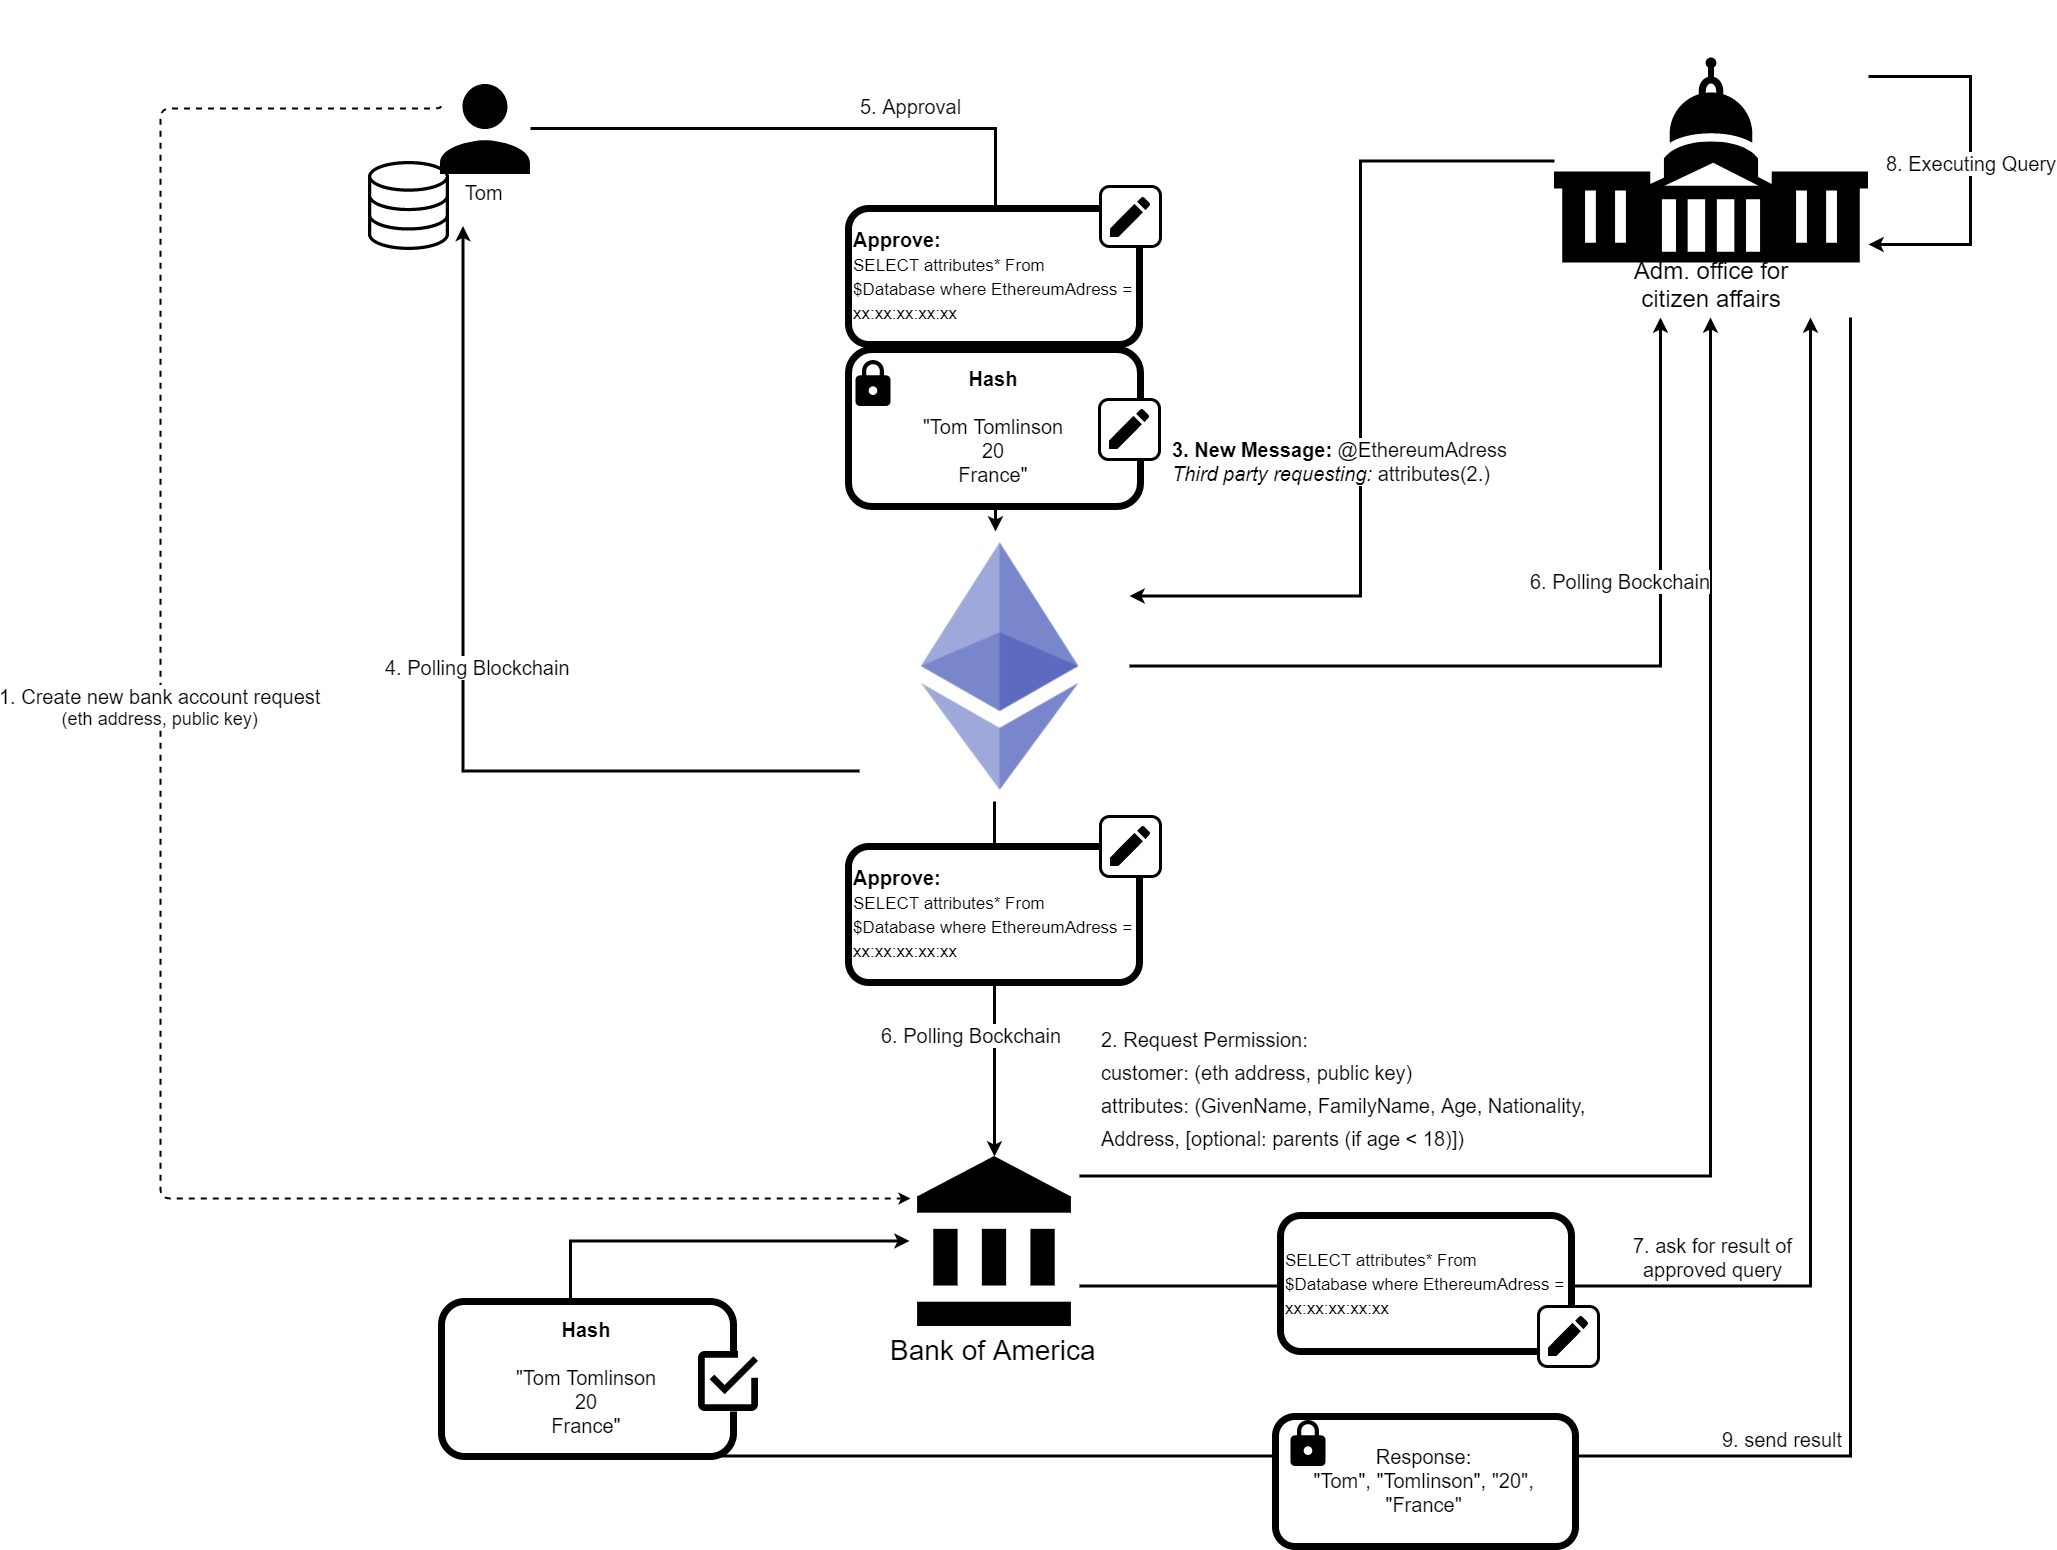
\includegraphics[width=\textwidth]{concept/permission_request_bank.png}
\caption{Permission Request}
\label{fig:permission_request}
\end{figure}

\subsection{Closures}
%Create closure figure in draw.io and insert here
\begin{comment}
\begin{figure}[ht]
\centering
\includegraphics[width=\textwidth]{concept/closure.png}
\caption{Closure}
\label{fig:closure}
\end{figure}
\end{comment}

\subsection{Changing Attributes}

\begin{figure}[ht]
\centering
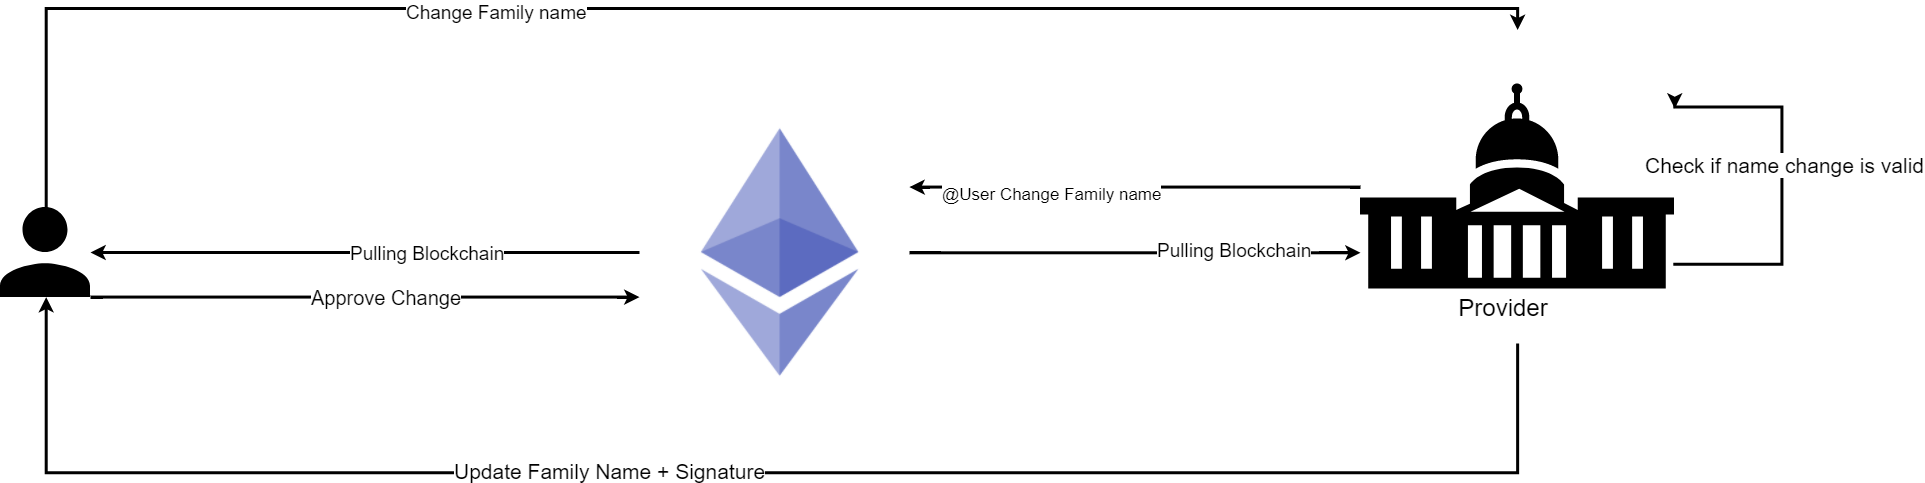
\includegraphics[width=\textwidth]{concept/change_attribute.png}
\caption{Change attribute}
\label{fig:change_attribute}
\end{figure}


Lets have a user Bob Bobsen who has recently married Alice Alison. Since Bob wants to change his family name to Bob Alison this information needs to be updated in our system. To do so he sends an "Update-Familiy-Name-Request" with his new family name to the corresponding identity provider. They on the other hand, can now verify this new claim by checking Bob's marrital status. If all information match Bobs claim, the identity provider publishes a "Change-Family-Name-Claim" transaction into the blockchain to notify all concerning parties about this change. 
Bob then pulls the blockchain, verifies the transaction code and approves the change by publishing his approval to the blockchain. The government permanently changes Bobs name in their database and sends the changes to Bob so that he can store the same changes in his local database. 
Each provider also holding bobs family name can then query the identity provider for Bobs new name, if Bob allowed that entity to query for his name.
The process described above will be processed in the same way when a third party requests a change of a claim. Bob on the other hand needs to explicitly approve this change. To model both transactions in the same way we hide who triggered the information change.

\subsection{Evaluation}

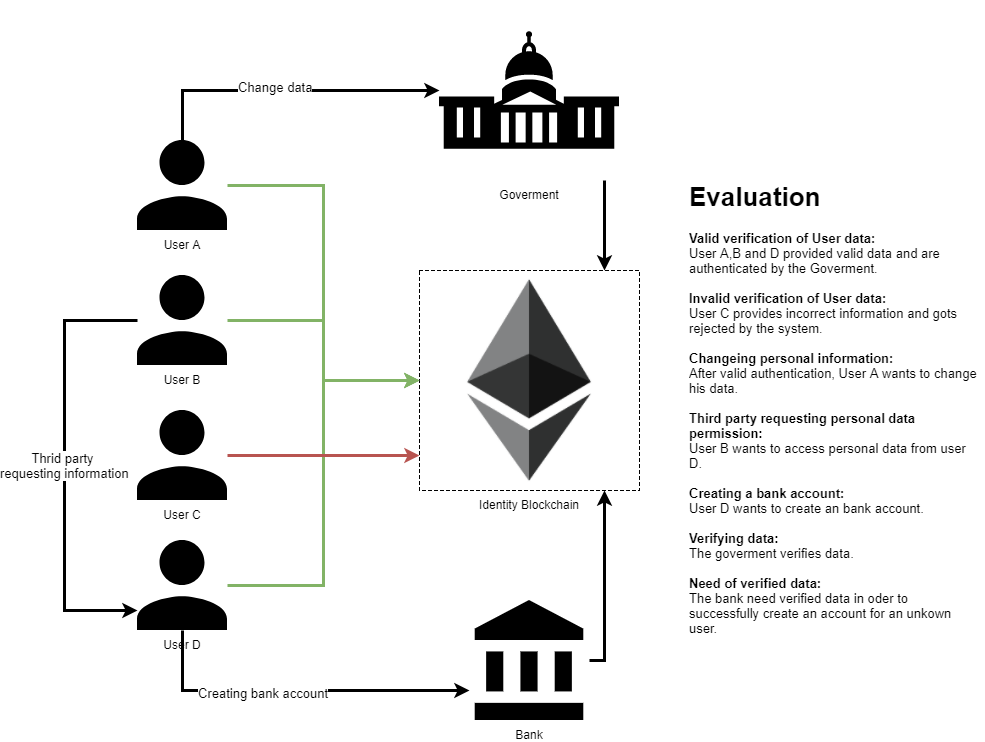
\includegraphics[width=\textwidth]{concept/evaluation.png}
 
\section{Use cases}

\subsection{Change a claim}
